\documentclass{beamer}

\mode<presentation> {

\usetheme{Madrid}

}
\usepackage{graphicx,wrapfig,lipsum}
\usepackage{graphicx}
\usepackage{booktabs}
\usepackage{subcaption}
\usepackage[nodayofweek,level]{datetime}
\usepackage{algpseudocode}
\usepackage{algorithm2e, float}
\usepackage{tikz}
\usepackage{tikz-3dplot}
\usetikzlibrary{arrows,patterns}

\tikzstyle{block} = [draw, fill=blue!20, rectangle, 
    minimum height=3em, minimum width=6em]
\tikzstyle{sum} = [draw, fill=white, circle, node distance=1cm]
\tikzstyle{input} = [coordinate]
\tikzstyle{output} = [coordinate]
\tikzstyle{pinstyle} = [pin edge={to-,thick,black}]
\tdplotsetmaincoords{70}{20}

\SetKwInOut{Parameter}{Parameters}
\newdate{date}{10}{09}{2018}
\date{\displaydate{date}}
\newcommand{\PaperLecturer} {Prof. Dr. Paul G. Pl\"oger}
\newcommand{\SecondAdvisor} {Prof. Dr. Roustiam Chakirov}
\newcommand{\ThirdAdvisor} {M.Sc. Sven Schneider}

%----------------------------------------------------------------------------------------
%	TITLE PAGE
%----------------------------------------------------------------------------------------

\title[Master Thesis]{Accurate trajectory tracking on the KUKA
youBot manipulator: Computed-torque control and Friction compensation} 

\author{Jeyaprakash Rajagopal}
\institute[MT]
{
%University of Applied Sciences Bonn-Rhein-Sieg \\
\includegraphics[scale=0.05]{images/logo} 
\hfill
\includegraphics[scale=0.04]{images/b-it.pdf}
\\
\medskip
\vspace{0.2cm}
\textit{\Large \textbf{Supervisors}} \\
\vspace{0.2cm}\large\PaperLecturer \\
\vspace{0.01cm}\large\SecondAdvisor \\
\vspace{0.01cm}\large\ThirdAdvisor
\vspace{0.2cm}
\date{\displaydate{date}}
}
\def\Arrow{\raisebox{-.5\height}{\scalebox{1}{$\Longrightarrow$}}}
\setbeamertemplate{caption}[numbered]

\begin{document}

\begin{frame}
	\titlepage
\end{frame}

\renewcommand{\baselinestretch}{1.5}

%----------------------------------------------------------------------------------------
%	PRESENTATION SLIDES
%----------------------------------------------------------------------------------------

%------------------------------------------------
\section{Motivation}
\begin{frame}
	\frametitle{Motivation}
\begin{figure}[H]
	\includegraphics[trim=0 350 0 350,width=0.8\linewidth]{images/tiles}
	\caption{Filling gaps between tiles}
\end{figure}	
\vspace{-1cm}
	\begin{itemize}
		\item Filling the gaps with waterproof liquid in between tiles
		\item Welding and surgical tasks also require high-precision tracking
		\item Don't damage environment and the robot
	\end{itemize}
\end{frame}

\section{Related work}
\begin{frame}
	\frametitle{Related work}
	\vspace{-0.5cm}
	\begin{itemize}
		\item Newton-Euler formulation has been used mostly in rigid-body algorithms~\cite{p3}~\cite{p4}~\cite{p5}~\cite{p8}
		\item In previous work~\cite{p7}, geometrical relation semantics were constructed in the numerical level and the parameter identification is incomplete
		\item Parameters identification methods based on the modified Newton-Euler formulation were proposed by~\cite{p3}~\cite{p6}
		\item The friction modeling and compensation brings us close to the complete dynamics~\cite{p10}~\cite{p11}
		\item Computed-torque control scheme has been proposed by many authors~\cite{p2}~\cite{p9} which discuss progress towards complete dynamics
	\end{itemize}
\end{frame}

\section{Problem formulation}
\begin{frame}
	\frametitle{Problem formulation}
	\vspace{-0.5cm}
	\begin{itemize}
		\item Achieving accurate trajectory tracking in a non-linear system is difficult due to the following
		\begin{itemize}
		\item Complexity of the dynamics
		\item Uncertainties 
		\end{itemize}
		\item So, manipulator dynamics has to be considered in control scheme
		\item Construction of rigid-body algorithms has to consider the following
		\begin{itemize}
		\item Geometric relations between rigid-bodies has to involve semantics checking in addition to numerical computations
		\item Rigid-body algorithm's with this standard check avoids logical error, and perform meaningful operations
		\end{itemize}
		\item Requirement of excitation trajectories for parameter identification 
	\end{itemize}
\end{frame}

\section{Approach}

\begin{frame}
	\frametitle{Approach}
\begin{figure}
\centering
\begin{minipage}{.45\textwidth}
  \centering
  \includegraphics[trim=0 300 0 250,width=0.9\linewidth]{images/tiles_robot}
  \captionof{figure}{Manipulation task}
\end{minipage}
\hspace{-1cm}
\begin{minipage}{.45\textwidth}
  \centering
\vspace{2cm}
  \includegraphics[trim=0 400 0 400,width=1.3\linewidth]{images/controlonly}
  \captionof{figure}{Closed-loop system}
\end{minipage}
\end{figure}		
	\begin{itemize} 
	\item Problem: It could damage the environment and robot due to 
	\begin{itemize}
	\item system is non-linear
	\item compromise on performance due to uncertainties
	\end{itemize}
\pause
	\item Solution: Accounting manipulator dynamics and manipulator configuration
	\end{itemize}
\end{frame}

\begin{frame}
\frametitle{Basic and alternate approach}
\vspace{-0.2cm}
\begin{center}
\tikz \node [scale=0.65, inner sep=0] {
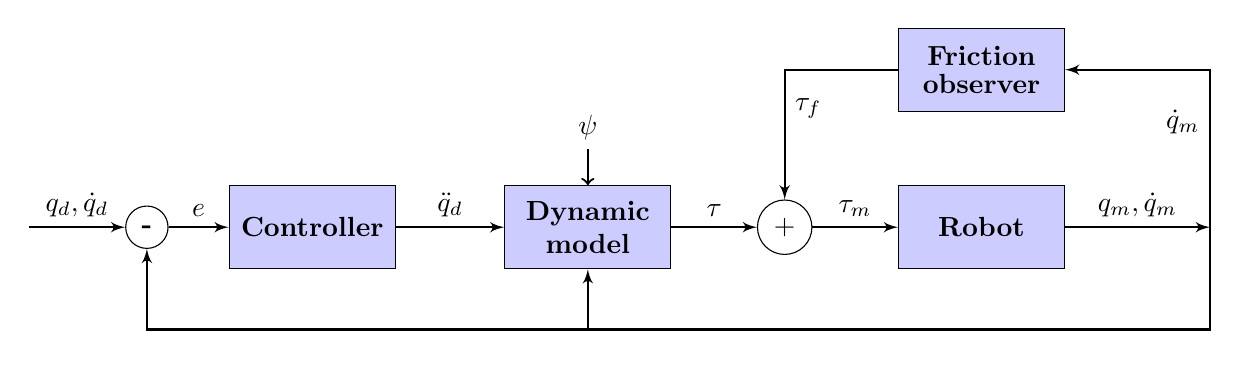
\begin{tikzpicture}[auto,node distance=2cm,>=latex']
    \node [input, name=input] {};
    \node [sum, right of=input, node distance=1.5cm] (minus) {\textbf{-}};
    \node [block, right of=minus, node distance=2.1cm] (control) {\textbf{Controller}};
    \node [block, right of=control, node distance=3.5cm, pin={[pinstyle]above: $\psi$}] (model){\textbf{\shortstack{Dynamic\\ model}}};
    \node [sum, right of=model, node distance=2.5cm](summation) {\textbf{$+$}};
    \node [block, right of=summation,
            node distance=2.5cm] (robot) {\textbf{Robot}};
    \node [block, above of=robot, node distance=2cm](friction) {\textbf{\shortstack{Friction\\ observer}}};
	\node [output, right of=robot, node distance=2.9cm](output){};
	\draw [->,thick] (input) -- node {$q_d, \dot{q}_d$} (minus);
	\draw [->,thick] (minus) -- node {$e$} (control);
	\draw [->,thick] (control) -- node {$\ddot{q}_d$} (model);	
    \draw [->,thick] (model) -- node {$\tau$} (summation);
    \draw [->,thick] (summation) -- node {$\tau_m$} (robot);    
	\draw [->,thick] (friction) -- ++ (-2.0, 0) -| node [pos=0.65] {$\tau_f$} (summation);	
    \draw [->,thick] (robot) -- node[pos=0.5] {$q_m, \dot{q}_m$} (output);
	\draw [->,thick] (output) -- ++ (0,-1.3) |- node [pos=0.4] {$\dot{q}_m$} (friction);
	\draw [->,thick] (output) -- ++ (0,-1.3) -| node [] {} (minus);
	\draw [->,thick] (output) -- ++ (0,-1.3) -| node [] {} (model);
\end{tikzpicture}
};
\captionof{figure}{Basic approach: inaccurate model parameters}
\label{fig:basicapproach}
\end{center}
\vspace{-0.5cm}
\begin{center}
\tikz \node [scale=0.65, inner sep=0] {
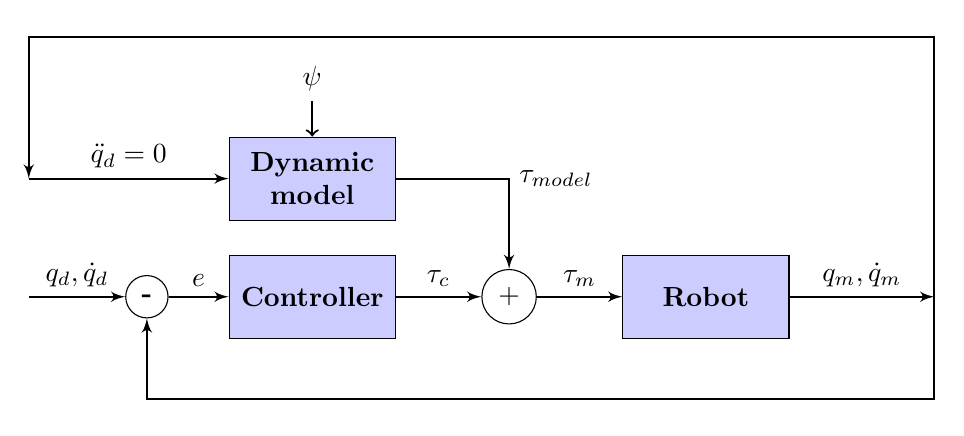
\begin{tikzpicture}[auto, node distance=2cm,>=latex']
    \node [input, name=input] {};
    \node [input, above of=input, name=input1, node distance=1.5cm] {};
    \node [sum, right of=input, node distance=1.5cm] (minus) {\textbf{-}};
    \node [block, right of=minus, node distance=2.1cm] (control) {\textbf{Controller}};
    \node [block, above of=control, node distance=1.5cm, pin={[pinstyle]above: $\psi$}] (model){\textbf{\shortstack{Dynamic\\ model}}};
    \node [sum, right of=control, node distance=2.5cm](summation) {\textbf{$+$}};
    \node [block, right of=summation,
            node distance=2.5cm] (robot) {\textbf{Robot}};
	\node [output, right of=robot, node distance=2.9cm](output){};
	\draw [->,thick] (input) -- node {$q_d, \dot{q}_d$} (minus);
	\draw [->,thick] (input1) -- node {$\ddot{q}_d=0$} (model);
	\draw [->,thick] (minus) -- node {$e$} (control);
	\draw [->,thick] (control) -- node {$\tau_c$} (summation);	
    \draw [->,thick] (model) -| node {$\tau_{model}$} (summation);
    \draw [->,thick] (summation) -- node {$\tau_m$} (robot);    
    \draw [->,thick] (robot) -- node[pos=0.5] {$q_m, \dot{q}_m$} (output);
	\draw [->,thick] (output) -- ++ (0,-1.3) -| node [] {} (minus);
	\draw [->,thick] (output) -- ++ (0, 3.3) -| node [] {} (input1);
\end{tikzpicture}
};
\captionof{figure}{Alternate approach with simple computed-torque control}
\label{fig:alternateapproach}
\end{center}
\end{frame}

\begin{frame}
	\frametitle{Approach}
\begin{center}
\tikz \node [scale=0.9, inner sep=0] {
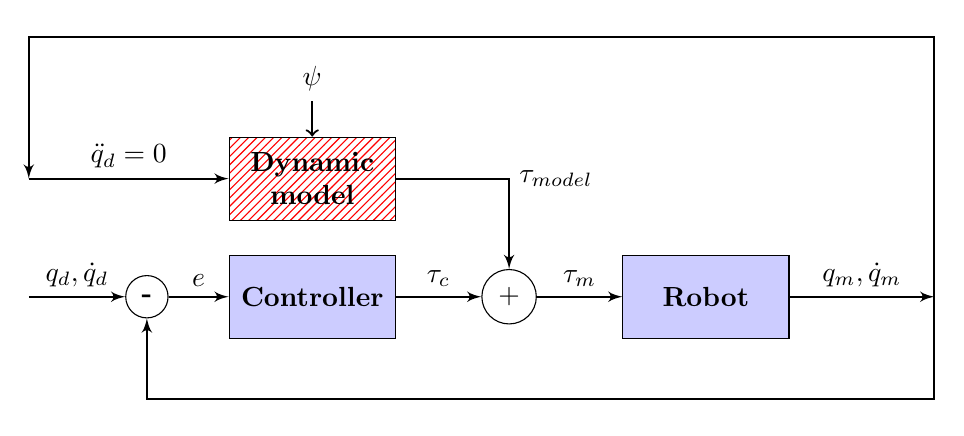
\begin{tikzpicture}[auto, node distance=2cm,>=latex']
    \node [input, name=input] {};
    \node [input, above of=input, name=input1, node distance=1.5cm] {};
    \node [sum, right of=input, node distance=1.5cm] (minus) {\textbf{-}};
    \node [block, right of=minus, node distance=2.1cm] (control) {\textbf{Controller}};
    \node [block,pattern=north east lines,pattern color=red, above of=control, node distance=1.5cm, pin={[pinstyle]above: $\psi$}] (model){\textbf{\shortstack{Dynamic\\ model}}};
    \node [sum, right of=control, node distance=2.5cm](summation) {\textbf{$+$}};
    \node [block, right of=summation,
            node distance=2.5cm] (robot) {\textbf{Robot}};
	\node [output, right of=robot, node distance=2.9cm](output){};
	\draw [->,thick] (input) -- node {$q_d, \dot{q}_d$} (minus);
	\draw [->,thick] (input1) -- node {$\ddot{q}_d=0$} (model);
	\draw [->,thick] (minus) -- node {$e$} (control);
	\draw [->,thick] (control) -- node {$\tau_c$} (summation);	
    \draw [->,thick] (model) -| node {$\tau_{model}$} (summation);
    \draw [->,thick] (summation) -- node {$\tau_m$} (robot);    
    \draw [->,thick] (robot) -- node[pos=0.5] {$q_m, \dot{q}_m$} (output);
	\draw [->,thick] (output) -- ++ (0,-1.3) -| node [] {} (minus);
	\draw [->,thick] (output) -- ++ (0, 3.3) -| node [] {} (input1);
\end{tikzpicture}
};
\captionof{figure}{Alternate approach}
%\label{fig:alternateapproach}
\end{center}
\begin{itemize}
\item Let's have a look into dynamic model of the robot manipulator
\end{itemize}
\end{frame}

\begin{frame}
	\frametitle{Dynamic model I}
	\begin{itemize}
		\item The general equation of motion~\cite{p2} can be given as
\begin{equation}
\label{eq:dynamics}
\tau_{model} = M(q, \psi) \overbrace{\ddot{q}}^{Joining point} + \underbrace{C(q, \dot{q}, \psi)\dot{q} + N(q,\dot{q}, \psi)}_{non-linear}
\end{equation}
		\item where M, C and N are non-linear functions of $\psi$ (model parameters)
		\item $\ddot{q}$ can be replaced with linear controller i.e. PID~\cite{p12}
		\item The non-linear terms C, N are handled by dynamic model which includes friction
		\item This work uses \textbf{Inverse Dynamics }solver from Orocos KDL~\cite{p4}
	\end{itemize}
\end{frame}

\begin{frame}
	\frametitle{Dynamic model II - findings}
	\vspace{-0.5cm}
	\begin{itemize}
	\item Kinematic chain of youBot manipulator is constructed in KDL
	\item Dynamic model parameters $\psi$ are taken from manufacturers~\cite{p13} defined w.r.t. reference frame
	\item Center of mass and inertial frames are depicted w.r.t. reference frame
\begin{figure}
\centering
\begin{minipage}{.4\textwidth}
  \centering
  \includegraphics[trim=0 20 0 20,width=0.9\linewidth]{images/kdl_segment}
  \captionof{figure}{Segment image~\cite{p4}}
\end{minipage}
\pause
\begin{minipage}{.4\textwidth}
  \centering
\vspace{-2.3cm}
  \includegraphics[trim=0 300 0 0,width=1.0\linewidth]{images/kdl_segment_modified}
  \captionof{figure}{Modified}
\end{minipage}
\end{figure}	
	\item But implementation considers tip frame as reference
	\item Relations between rigid-bodies are defined implicitly
	\end{itemize}
\end{frame}

\begin{frame}
	\frametitle{Dynamic model III}
	\vspace{-0.5cm}
	\begin{itemize}
	\item In previous work~\cite{p7}, implementation was based on coordinate computations without semantics checkings
	\item Geometric relation semantics of rigid-body algorithms are analyzed
	\item It includes pose, motion and force related semantics
	\item Why is it important to include semantics checking?
	\begin{itemize}
	\item Rigid body conventions differ from one author to another
	\item To avoid logical errors in rigid body algorithm construction
	\item i.e. Transforming twists between rigid bodies requires a common point and same coordinate frame
	\end{itemize}
	\end{itemize}
\end{frame}

\begin{frame}
	\frametitle{Dynamic model IV}
	\vspace{-0.7cm}
	\begin{figure}
\centering
\begin{minipage}{.4\textwidth}
  \centering
  \captionof{figure}{KDL segment}
  \vspace{-0.5cm}
  \includegraphics[trim=0 100 0 220,width=1.1\linewidth]{images/kdl_rigidbodyi}
\end{minipage}
\begin{minipage}{.4\textwidth}
  \centering
\vspace{-2cm}
  \captionof{figure}{Featherstone}
  \vspace{-0.5cm}
  \includegraphics[trim=0 350 0 200,width=1.1\linewidth]{images/featherstone_rigidbodyi}
\end{minipage}
\end{figure}	
\vspace{-1.6cm}
\begin{minipage}{.45\textwidth}
  \centering
	\begin{itemize}
	\item t: Position($tip_i, joint_i$) \\ R: Rotation($[tip_i], [root_i]$)
	\item V$_J$ = Twist($joint_i | Body_i,$ \\$Body_{i-1}, [root_i]$)
	\end{itemize}
\end{minipage}
\begin{minipage}{.45\textwidth}
  \centering
	\begin{itemize}
	\item t: Position($tip_i, joint_i$) \\ R: Rotation($[root_i], [tip_i]$)
	\item V$_J$ = Twist($root_i | Body_i,$ \\$Body_{i-1}, [root_i]$)
	\end{itemize}
\end{minipage}
\vspace{-1cm}
\begin{figure}[H]
	\includegraphics[trim=0 250 0 250,width=0.7\linewidth]{images/transform_kdl_featherstone}
\end{figure}
\end{frame}

\begin{frame}
	\frametitle{Parameter identification - Excitation trajectories}
	\begin{itemize}
	\item Trajectory parameterization and optimization is needed to get excitation trajectories~\cite{p6}
	\item Finite Fourier series is used to get parameterized trajectories
	\item Optimizing an objective function $K^TK$ over the coefficients a, b, q(0)
	\begin{itemize}
		\item where q(0) represents initial position of the joint
		\item a, b are the coefficients that covers the workspace of the joint
		\item Constraints are $q, \dot{q}, \ddot{q}$ within the joint limits and no collision constraint
	\end{itemize}
	\end{itemize}
\end{frame}

\begin{frame}
	\frametitle{Approach}
\begin{center}
\tikz \node [scale=0.9, inner sep=0] {
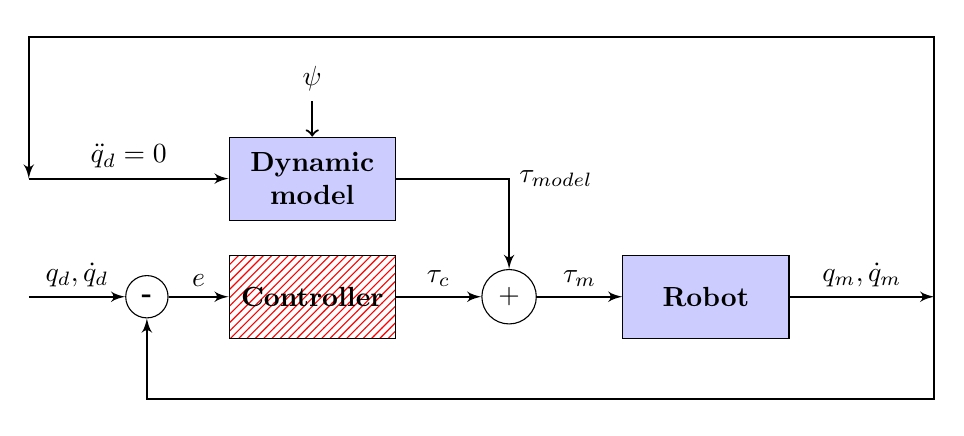
\begin{tikzpicture}[auto, node distance=2cm,>=latex']
    \node [input, name=input] {};
    \node [input, above of=input, name=input1, node distance=1.5cm] {};
    \node [sum, right of=input, node distance=1.5cm] (minus) {\textbf{-}};
    \node [block,pattern=north east lines,pattern color=red, right of=minus, node distance=2.1cm] (control) {\textbf{Controller}};
    \node [block, above of=control, node distance=1.5cm, pin={[pinstyle]above: $\psi$}] (model){\textbf{\shortstack{Dynamic\\ model}}};
    \node [sum, right of=control, node distance=2.5cm](summation) {\textbf{$+$}};
    \node [block, right of=summation,
            node distance=2.5cm] (robot) {\textbf{Robot}};
	\node [output, right of=robot, node distance=2.9cm](output){};
	\draw [->,thick] (input) -- node {$q_d, \dot{q}_d$} (minus);
	\draw [->,thick] (input1) -- node {$\ddot{q}_d=0$} (model);
	\draw [->,thick] (minus) -- node {$e$} (control);
	\draw [->,thick] (control) -- node {$\tau_c$} (summation);	
    \draw [->,thick] (model) -| node {$\tau_{model}$} (summation);
    \draw [->,thick] (summation) -- node {$\tau_m$} (robot);    
    \draw [->,thick] (robot) -- node[pos=0.5] {$q_m, \dot{q}_m$} (output);
	\draw [->,thick] (output) -- ++ (0,-1.3) -| node [] {} (minus);
	\draw [->,thick] (output) -- ++ (0, 3.3) -| node [] {} (input1);
\end{tikzpicture}
};
\captionof{figure}{Alternative approach}
%\label{fig:alternateapproach}
\end{center}
\begin{itemize}
\item Let's have a look into controller
\item Computed-torque control runs at $\approx$ 1 KHz due to EtherCAT sampling constraint
\end{itemize}
\end{frame}

\begin{frame}
	\frametitle{Safety controller}
	\vspace{-0.5cm}
	\begin{itemize}
		\item Safety of the hardware is the primary focus to save equipments
		\item Before commanding \textbf{torque} to manipulator joints, three different checks are performed
		\begin{itemize}
			\item \textbf{Position }limit check based on measured joint positions
			\item \textbf{Velocity }limit check based on measured joint velocities
			\item \textbf{Torque }limit check based on measured joint torques
		\end{itemize}
		\item If any of these check fails controller sets joint velocities to zero and quits
		\item Artificial joint limits are imposed and clamping
	\end{itemize}
\end{frame}

\begin{frame}
	\frametitle{Cascade PI control I}
	\vspace{-0.5cm}
	\begin{itemize}
		\item The outer-loop controller is position PI and inner-loop is velocity PI
\begin{center}
\tikz \node [scale=0.8, inner sep=0] {
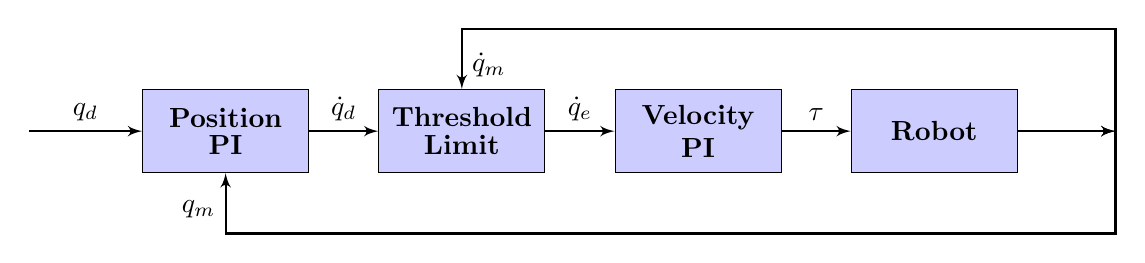
\begin{tikzpicture}[auto, node distance=2cm,>=latex']
    \node [input, name=input] {};
    \node [block, right of=input, node distance=2.5cm] (pcontrol) {\textbf{\shortstack{Position\\ PI}}};
    \node [block, right of=pcontrol, node distance=3cm] (limitcheck) {\textbf{\shortstack{Threshold\\ Limit}}};
    \node [block, right of=limitcheck, node distance=3cm](vcontrol) {\textbf{\shortstack{Velocity\\ PI}}};
    \node [block, right of=vcontrol,
            node distance=3.0cm] (robot) {\textbf{Robot}};
	\node [output, right of=robot, node distance=2.3cm](output){};
	\node [output, right of=robot, node distance=2.3cm](output1){};
	\draw [->,thick] (input) -- node {$q_d$} (pcontrol);
	\draw [->,thick] (pcontrol) -- node {$\dot{q}_d$} (limitcheck);
	\draw [->,thick] (limitcheck) -- node {$\dot{q}_e$} (vcontrol);
	\draw [->,thick] (vcontrol) -- node {$\tau$} (robot);
    \draw [->,thick] (robot) -- node[pos=0.55] {} (output);
    \draw [->,thick] (robot) -- node[pos=0.55] {} (output);
	\draw [->,thick] (output) -- ++ (0,-1.3) -| node [pos=0.7] {$q_m$} (pcontrol);
	\draw [->,thick] (output1) -- ++ (0,1.3) -| node [pos=0.8] {$\dot{q}_m$} (limitcheck);	
\end{tikzpicture}
};
\captionof{figure}{Cascade PI controller}
\end{center}
		\item Position controller output is fed as an input to velocity PI controller
		\begin{equation}
\dot{q}_d = q_e\cdot K_p + \sum q_e\cdot K_i 
\end{equation}
		\item Control output of position PI is fed to inner-loop
	\end{itemize}
\end{frame}

\begin{frame}
	\frametitle{Cascade PI control II}
	\begin{itemize}
		\item Produces higher velocity if disturbances are not handled	
		\item Limiting velocity of the joint 
		\begin{equation}
			\dot{q}_e = limit(\dot{q}_d - \dot{q}_m)
		\end{equation}				
		\item Cascaded PI control along with gravity compensation looks like
\begin{equation}
\tau = \overbrace{(\dot{q}_e\cdot K_p + \sum \dot{q}_e\cdot K_i)}^{Control Variable} + \overbrace{\tau_g(q)}^{Torque due to gravity} + bias
\end{equation}
	\item The above equation specifies computed-torque control scheme
	\end{itemize}	
\end{frame}

\begin{frame}
	\frametitle{Friction observer}
	\vspace{-0.2cm}
	\begin{itemize}
		\item Friction is a non-linear phenomenon that needs to be modeled and it can be classified into
		\begin{itemize}
			\item Static friction is applied when joint is in equilibrium state
			\item Coulomb friction is applied when joint is at motion			\end{itemize}
	\end{itemize}
	\vspace{-0.45cm}
\begin{figure}[H]
	\centering
	\caption{Simple model of friction}
	\includegraphics[trim=0 0 0 220,width=0.35\paperwidth, height=0.55\paperheight]{images/friction_staticandcoulomb}
\end{figure}	
\end{frame}

\begin{frame}
	\frametitle{Flow diagram and libraries used}
	\vspace{-0.2cm}
\begin{figure}[H]
	\centering
	\includegraphics[trim=0 150 0 75,width=0.5\linewidth]{images/softwaredesign}
	\caption{Software flow}
\end{figure}	
\end{frame}
%--------------------------------------------------------------------------
\section{Experimentation}
%--------------------------------------------------------------------------
\begin{frame}
	\frametitle{Experimentation}
	\centering
	\begin{minipage}{0.4\textwidth}
	\begin{figure}[H]
		\includegraphics[width=0.7\linewidth]{images/youbot.jpg}
	\end{figure}
	\end{minipage} \hfill
	\begin{minipage}{0.55\textwidth}	
	Experimentation steps
	\begin{itemize}
	\item{Safety controller on base and arm}
	\item{Tuning controller gains}
	\item{Cascade PI control}
	\item{Gravity compensation}
	\item{Validation of model-based controller}
	\end{itemize}
	\end{minipage}
\end{frame}

\begin{frame}
	\frametitle{Empirical tuning of controller gains}
\begin{figure}
\centering
\begin{minipage}{.45\textwidth}
  \centering
  \includegraphics[trim=0 0 0 0,width=0.9\linewidth]{images/joint4_innerloop_0pt5rads}
  \captionof{figure}{Velocity PI tuning}
\end{minipage}
\begin{minipage}{.45\textwidth}
  \centering
  \includegraphics[trim=0 0 0 0,width=0.9\linewidth]{images/joint4_outerloop_0pt5rad}
  \captionof{figure}{Position PI tuning}
\end{minipage}
\end{figure}	
\begin{itemize}
\item Inner-loop controller is tuned at first then outer-loop
\item Increase P-gain till it reaches the set-point
\item Gradually increase I-gain till steady-state error is close to zero
\end{itemize}
\end{frame}

\begin{frame}
	\frametitle{Validation of computed-torque controller}
	\centering
\begin{minipage}{.45\textwidth}
\begin{figure}[H]
	\centering
	\includegraphics[trim=0 0 0 0,width=0.45\paperwidth, height=0.45\paperheight]{images/sinewave}
	\caption{Analytical trajectory}
\end{figure}		
\end{minipage}
\hfill
\begin{minipage}{.45\textwidth}
\begin{itemize}
	\item Simple sine wave is selected
	\item It is simpler to derive the velocity from q
	\item Compute maximum and minimum velocity of joints
	\item To validate the model-based controller
\end{itemize}
\end{minipage}
\end{frame}


\begin{frame}
	\frametitle{Validation of computed-torque controller}
\vspace{-0.3cm}
\begin{figure}
\centering
\begin{minipage}{.45\textwidth}
  \centering
  \includegraphics[trim=0 0 0 0,width=0.9\linewidth]{images/joint4_trajectory}
  %\captionof{figure}{Joint 4 validation}
\end{minipage}
\begin{minipage}{.45\textwidth}
  \centering
  \includegraphics[trim=0 0 0 0,width=0.85\linewidth]{images/joint5_trajectory}
  %\captionof{figure}{Joint 5 validation}
\end{minipage}
\end{figure}	
\vspace{-0.4cm}
\begin{figure}
\centering
\begin{minipage}{.45\textwidth}
  \centering
  \includegraphics[trim=0 0 0 0,width=0.9\linewidth]{images/joint4_trajectoryerror}
  %\captionof{figure}{Joint 4 error}
\end{minipage}
\begin{minipage}{.45\textwidth}
  \centering
  \includegraphics[trim=0 0 0 0,width=0.9\linewidth]{images/joint5_trajectoryerror}
  %\captionof{figure}{Joint 5 error}
\end{minipage}
\end{figure}	

\end{frame}

\begin{frame}
	\frametitle{Model and controller torques}
		\centering
\begin{minipage}{.45\textwidth}
\begin{figure}
\centering
  \includegraphics[trim=0 0 0 0,width=1.2\linewidth]{images/joint4_ratio}
\end{figure}	
\end{minipage}
\hfill
\begin{minipage}{.45\textwidth}
\begin{itemize}
\item Model has no high-frequency noises in gravity torques
\item Controller handles disturbances
\end{itemize}
\end{minipage}
\end{frame}

%--------------------------------------------------------------------------
\section{Conclusions and Future work}
\begin{frame}
	\frametitle{Conclusions I}
	\vspace{-0.3cm}
	\begin{itemize}
		\item Attempt to achieve complete dynamics which improves the performance of computed-torque control
		\item Kinematic chain of youBot manipulator is constructed manually
	\item The basic friction model that comprises static, Coulomb friction is implemented and compensation terms are added in dynamic model 
		\item Safety controller ensures the safety of the robotic joint with an acceptable delay in response
		\item Empirical tuning of the controller gains
	\end{itemize}
\end{frame}

\begin{frame}
	\frametitle{Conclusions II}
	\begin{itemize}
		\item Controller is implemented on youBot base due to the semantic mismatches between Simbody and KDL
		\item Cascaded PI controller in youBot manipulator runs in approximately 1 KHz
		\item Gravity compensation is achieved with model-based controller
		\item Model-based control scheme is validated by using analytical trajectories
		\item In spite of inaccurate model parameters, the proposed control scheme produces accurate tracking with some deviations 
	\end{itemize}
\end{frame}
%--------------------------------------------------------------------------
\begin{frame}
\frametitle{Future work}
\begin{itemize}
	\item Geometric relation semantics correction and identification 
	\item The basic approach can be used once accurate model parameters are identified
	\item Safety controller has to be adapted to check joint constraints actively than defining a static value
	\item Tuning controller gains based on auto-tuning procedures
	\item Inclusion of D-term increases stability 
	\item Controller's performance can be improved in a hard real-time operating systems
\end{itemize}
\end{frame}

%--------------------------------------------------------------------------
\setbeamertemplate{bibliography item}[text]
\section{References}
\begin{frame}
	\frametitle{References I}
	\footnotesize{
	\begin{thebibliography}{99} 
	\bibitem[1]{p1} KUKA youBot developers, Dynamic robot model . \emph{online at \url{http://www.youbot-store.com/developers/kuka-youbot-kinematics-dynamics-and-3d-model-81}, 2018}.

	\bibitem[2]{p2} Benjamin Keiser,  Elias M\"uggler, Matthias F\"assler, Davide Scaramuzza, Stephan Huck, and John Lygeros. Torque control of a kuka youbot arm.  (2013) \emph{source online at \url{https://github.com/uzh-rpg/rpg_youbot_torque_control/tree/master/youbot_arm_model}}.
	
	\bibitem[3]{p3} Chae H An, Christopher G Atkeson, and John M Hollerbach. Estimation of inertial parameters of rigid body links of manipulators. \emph{In Decision and Control, 1985 24th IEEE Conference on, volume 24, pages 990 to 995. IEEE, 1985}
		
	\bibitem[4]{p4} Ruben Smits, H Bruyninckx, and E Aertbeli¨en Kdl: Kinematics and dynamics library(2011).
	\emph{online at \url{http://www.orocos.org/kdl}}.

	\end{thebibliography}
	}
\end{frame}

\begin{frame}
	\frametitle{References II}
	\footnotesize{
	\begin{thebibliography}{99} 

	\bibitem[5]{p5} Roy Featherstone. Rigid body dynamics algorithms. 
	\emph{Springer, 2014}.
	
	\bibitem[6]{p6} Jan Swevers, Walter Verdonck, and Joris De Schutter. Dynamic model identification for industrial robots. \emph{IEEE Control Systems, 27(5):58{71, 2007}}
		
	\bibitem[7]{p7} Jeyaprakash Rajagopal. Dynamic robot model parameter identification via domain specific optimization. WS17 HBRS - Pl\"oger, Schneider Supervising, \emph{December, 2017}
	\bibitem[8]{p8} Sherman, Michael A and Seth, Ajay and Delp, Scott L. Simbody: multibody dynamics for biomedical research 2011. Procedia Iutam, \emph{Online at \url{https://simtk.org/projects/simbody}}
	\bibitem[9]{p9} C. H. An, C. G. Atkeson, J. D. Griffiths, and J. M. Hollerbach. Experimental evaluation of feedforward and computed torque control. IEEE Transactions on Robotics and Automation, \emph{5(3):368–373, Jun 1989}
\end{thebibliography}
	}
\end{frame}

\begin{frame}
	\frametitle{References III}
	\footnotesize{
	\begin{thebibliography}{99} 

	\bibitem[10]{p10} Olsson, Henrik and {\AA}str{\"o}m, Karl Johan and De Wit, Carlos Canudas and G{\"a}fvert, Magnus and Lischinsky, Pablo. Friction models and friction compensation, \emph{Eur. J. Control, 4(3):176–195, 1998}
	\bibitem[11]{p11} Ruiz, Miguel Corber{\'a}n, Haptic Teleoperation of the youBot with friction compensation for the base, \emph{PhD thesis, MA thesis. Departamento de Ingenier ́ıa de Sistema y Autom ́atica,
Universidad Carlos III de Madrid, 2012. URL: http://hdl. handle. net/10016/16267 (cit. on p. 168), 2012}
	\bibitem[12]{p12} W. K. Chung, L.-C. Fu, and T. Kr ̈oger. Motion Control, pages 163–194. \emph{Springer International Publishing, Cham, 2016.}-
	\bibitem[13]{p13} youBot developers. Dynamic robot model. \emph{online at - \url{https://www.youbot-store.com/developers/kuka-youbot-kinematics-dynamics-and-3d-model-81}, Nov 2016.}
\end{thebibliography}
	}
\end{frame}
%--------------------------------------------------------------------------
\begin{frame}
	\Huge{\centerline{Questions???}}
\end{frame}

\begin{frame}
	\Huge{\centerline{The End}}
\end{frame}
%--------------------------------------------------------------------------

\end{document}